% **** Szablon pracy magisterskiej, licencjackiej lub inżynierskiej ****

\documentclass[polish,12pt,twoside,a4paper]{report}

% *************** Definicje stylu dokumentu ***************

% *********************************************************************************
% W pliku tym zdefiniowany jest wygl¹d dokumentu.
% Zmiany tutaj nie s¹ konieczne o ile nie zamierzasz zmieniaæ wygl¹du dokumentu.
% *********************************************************************************

% *************** Za³adowanie pakietów ***************
\usepackage[a4paper,twoside,left=2.0cm,right=1.5cm,top=1.5cm,bottom=1.5cm]{geometry}
\usepackage[T1]{fontenc}
%\usepackage[cp1250]{inputenc}
\usepackage[utf8]{inputenc}
\usepackage[polish]{babel}
\usepackage{amsmath}
\usepackage{amsfonts}
\usepackage{graphicx}
\usepackage{graphics}
\usepackage{times}
\usepackage{indentfirst}%wciecia a nowych akapitach
\usepackage{listings}
\usepackage{url}
\usepackage{pgfgantt}
\usepackage[utf8]{inputenc}
\usepackage[T1]{fontenc}
\usepackage[polish]{babel}
\usepackage{pgfgantt}
\usepackage{float}
\usepackage{lmodern}
\usepackage{geometry}
\usepackage[colorlinks=true, linkcolor=black, urlcolor=black, citecolor=black]{hyperref}

\selectlanguage{polish}

%szerokoœœ wciêæ
\setlength{\parindent}{1.25cm}

%numeracja stron
\usepackage{fancyhdr}
\pagestyle{fancy}
\fancyhf{} % usun biezace ustawienia pagin
\fancyhead[LE,RO]{ }
\fancyhead[LO]{ }
\fancyhead[RE]{ }
\fancyfoot[LE,RO]{\small\thepage}
\fancyfoot[LO]{ }
\fancyfoot[RE]{ }
\renewcommand{\headrulewidth}{0.0pt}
\renewcommand{\footrulewidth}{0.0pt}
\addtolength{\headheight}{0.0pt} % pionowy odstep na kreske
\fancypagestyle{plain}{%
\fancyhead{} % usun p. górne na stronach pozbawionych
% numeracji (plain)
\renewcommand{\headrulewidth}{0.0pt} % pozioma kreska
}

% *************** Definicje niektórych kolorów ***************
\usepackage{color}

\definecolor{greenyellow}   {cmyk}{0.15, 0   , 0.69, 0   }
\definecolor{yellow}        {cmyk}{0   , 0   , 1   , 0   }
\definecolor{goldenrod}     {cmyk}{0   , 0.10, 0.84, 0   }
\definecolor{dandelion}     {cmyk}{0   , 0.29, 0.84, 0   }
\definecolor{apricot}       {cmyk}{0   , 0.32, 0.52, 0   }
\definecolor{peach}         {cmyk}{0   , 0.50, 0.70, 0   }
\definecolor{melon}         {cmyk}{0   , 0.46, 0.50, 0   }
\definecolor{yelloworange}  {cmyk}{0   , 0.42, 1   , 0   }
\definecolor{orange}        {cmyk}{0   , 0.61, 0.87, 0   }
\definecolor{burntorange}   {cmyk}{0   , 0.51, 1   , 0   }
\definecolor{bittersweet}   {cmyk}{0   , 0.75, 1   , 0.24}
\definecolor{redorange}     {cmyk}{0   , 0.77, 0.87, 0   }
\definecolor{mahogany}      {cmyk}{0   , 0.85, 0.87, 0.35}
\definecolor{maroon}        {cmyk}{0   , 0.87, 0.68, 0.32}
\definecolor{brickred}      {cmyk}{0   , 0.89, 0.94, 0.28}
\definecolor{red}           {cmyk}{0   , 1   , 1   , 0   }
\definecolor{orangered}     {cmyk}{0   , 1   , 0.50, 0   }
\definecolor{rubinered}     {cmyk}{0   , 1   , 0.13, 0   }
\definecolor{wildstrawberry}{cmyk}{0   , 0.96, 0.39, 0   }
\definecolor{salmon}        {cmyk}{0   , 0.53, 0.38, 0   }
\definecolor{carnationpink} {cmyk}{0   , 0.63, 0   , 0   }
\definecolor{magenta}       {cmyk}{0   , 1   , 0   , 0   }
\definecolor{violetred}     {cmyk}{0   , 0.81, 0   , 0   }
\definecolor{rhodamine}     {cmyk}{0   , 0.82, 0   , 0   }
\definecolor{mulberry}      {cmyk}{0.34, 0.90, 0   , 0.02}
\definecolor{redviolet}     {cmyk}{0.07, 0.90, 0   , 0.34}
\definecolor{fuchsia}       {cmyk}{0.47, 0.91, 0   , 0.08}
\definecolor{lavender}      {cmyk}{0   , 0.48, 0   , 0   }
\definecolor{thistle}       {cmyk}{0.12, 0.59, 0   , 0   }
\definecolor{orchid}        {cmyk}{0.32, 0.64, 0   , 0   }
\definecolor{darkorchid}    {cmyk}{0.40, 0.80, 0.20, 0   }
\definecolor{purple}        {cmyk}{0.45, 0.86, 0   , 0   }
\definecolor{plum}          {cmyk}{0.50, 1   , 0   , 0   }
\definecolor{violet}        {cmyk}{0.79, 0.88, 0   , 0   }
\definecolor{royalpurple}   {cmyk}{0.75, 0.90, 0   , 0   }
\definecolor{blueviolet}    {cmyk}{0.86, 0.91, 0   , 0.04}
\definecolor{periwinkle}    {cmyk}{0.57, 0.55, 0   , 0   }
\definecolor{cadetblue}     {cmyk}{0.62, 0.57, 0.23, 0   }
\definecolor{cornflowerblue}{cmyk}{0.65, 0.13, 0   , 0   }
\definecolor{midnightblue}  {cmyk}{0.98, 0.13, 0   , 0.43}
\definecolor{navyblue}      {cmyk}{0.94, 0.54, 0   , 0   }
\definecolor{royalblue}     {cmyk}{1   , 0.50, 0   , 0   }
\definecolor{blue}          {cmyk}{1   , 1   , 0   , 0   }
\definecolor{cerulean}      {cmyk}{0.94, 0.11, 0   , 0   }
\definecolor{cyan}          {cmyk}{1   , 0   , 0   , 0   }
\definecolor{processblue}   {cmyk}{0.96, 0   , 0   , 0   }
\definecolor{skyblue}       {cmyk}{0.62, 0   , 0.12, 0   }
\definecolor{turquoise}     {cmyk}{0.85, 0   , 0.20, 0   }
\definecolor{tealblue}      {cmyk}{0.86, 0   , 0.34, 0.02}
\definecolor{aquamarine}    {cmyk}{0.82, 0   , 0.30, 0   }
\definecolor{bluegreen}     {cmyk}{0.85, 0   , 0.33, 0   }
\definecolor{emerald}       {cmyk}{1   , 0   , 0.50, 0   }
\definecolor{junglegreen}   {cmyk}{0.99, 0   , 0.52, 0   }
\definecolor{seagreen}      {cmyk}{0.69, 0   , 0.50, 0   }
\definecolor{green}         {cmyk}{1   , 0   , 1   , 0   }
\definecolor{forestgreen}   {cmyk}{0.91, 0   , 0.88, 0.12}
\definecolor{pinegreen}     {cmyk}{0.92, 0   , 0.59, 0.25}
\definecolor{limegreen}     {cmyk}{0.50, 0   , 1   , 0   }
\definecolor{yellowgreen}   {cmyk}{0.44, 0   , 0.74, 0   }
\definecolor{springgreen}   {cmyk}{0.26, 0   , 0.76, 0   }
\definecolor{olivegreen}    {cmyk}{0.64, 0   , 0.95, 0.40}
\definecolor{rawsienna}     {cmyk}{0   , 0.72, 1   , 0.45}
\definecolor{sepia}         {cmyk}{0   , 0.83, 1   , 0.70}
\definecolor{brown}         {cmyk}{0   , 0.81, 1   , 0.60}
\definecolor{tan}           {cmyk}{0.14, 0.42, 0.56, 0   }
\definecolor{gray}          {cmyk}{0   , 0   , 0   , 0.50}
\definecolor{black}         {cmyk}{0   , 0   , 0   , 1   }
\definecolor{white}         {cmyk}{0   , 0   , 0   , 0   } 

% *************** Koniec definicji stylu dokumentu ***************


%definicja przydatnych poleceń
\newcommand{\wydzial}{KOLEGIUM INFORMATYKI STOSOWANEJ}
\newcommand{\kierunek}{Kierunek: INFORMATYKA}
\newcommand{\specjalnosc}{Specjalność: \textcolor{red}{Inżynieria Danych}}
\newcommand{\autor}{Wojciech Armata}
\newcommand{\album}{Nr albumu studenta w69760}
\newcommand{\temat}{System zarządzania pojazdami}
\newcommand{\promotor}{mgr inż. Ewa Żesławska}
\newcommand{\typpracy}{Praca projektowa programowanie obiekotwe C\#}
\newcommand{\miasto}{Rzeszów}
\newcommand{\rok}{2025}

\begin{document}

% *************** Włączenie definicji pierwszych stron ***************
% *************** Strony tytułowe ***************

% ************************************************************
% W tym miejscu znajduje sie definicja wyglądu pierwszych stron:
% strony tytułowej, strony z oświadczeniem o treści pracy
% i strony ze spisem treści
% ************************************************************
% *************** Strona tytułowa ***************
%umieszczenie logo i nazwy uczelni
\noindent
\parbox{65mm}{
\includegraphics[width=13.0cm, height=3.0cm]{logoWSIiZ}}

\vspace{10mm}
\begin{center}
{\Large{}\textbf{\wydzial}}
\end{center}
\vspace{10mm}
\noindent
\hspace{30mm}{\Large{}\textbf{\kierunek}}\\

\noindent
\hspace{30mm}{\Large{}\textbf{\specjalnosc}}
\vspace{30mm}
\begin{center}
	{\large{}\autor}\\
	{\large{}\album}\\
	\vspace{15pt}
	{\huge{}\textbf{\textit{\temat}}}\\
	\vspace{20pt}
	{\normalsize{}Prowadzący: \promotor}\\
	\vspace{100pt}
	{\LARGE{}\textbf{\typpracy}}\\
	\vspace{190pt}
	{\large{}\textbf{\miasto {} \rok}}
\end{center}

% pusta zawartość stopki - brak numeru strony
\thispagestyle{empty}

% *************** Strona z oświadczeniem o treści pracy ***************
\newpage
\text{}

\thispagestyle{empty}
\newpage


% *************** Spis treści ***************
\tableofcontents
% pusta zawartość stopki - brak numeru strony
\thispagestyle{empty}
\newpage

% *************** Koniec pliku front.tex ***************



% *************** Część główna pracy ***************
\chapter*{Wstęp}


Efektywne zarządzanie flotą pojazdów to kluczowy element sprawnego funkcjonowania firm i instytucji. Często jednak pojawiają się problemy z nieuporządkowanymi danymi, trudnościami w wyszukiwaniu pojazdów czy koniecznością ręcznego prowadzenia ewidencji, co prowadzi do dezorganizacji, opóźnień i zwiększonego ryzyka błędów.  

Stworzony system to aplikacja konsolowa, która usprawnia te procesy, zapewniając wygodne i uporządkowane zarządzanie danymi o pojazdach. Umożliwia szybkie dodawanie, edytowanie, usuwanie oraz wyszukiwanie pojazdów na podstawie numeru rejestracyjnego lub typu. Oprócz tego pozwala generować statystyki, co ułatwia analizę floty i podejmowanie decyzji związanych z jej eksploatacją.  

Kluczowym elementem systemu jest integracja z bazą SQL oraz obsługa plików, co zapewnia trwałość i bezpieczeństwo danych. Dzięki temu użytkownicy mają stały dostęp do aktualnych informacji i mogą skutecznie zarządzać flotą. Aplikacja jest prosta w obsłudze, niezawodna i gotowa do dalszej rozbudowy. To praktyczne narzędzie dla firm, które chcą efektywnie kontrolować swoje zasoby transportowe bez konieczności korzystania z rozbudowanych systemów z interfejsem graficznym.




\addcontentsline{toc}{chapter}{Wstęp}
\newpage
% ********** Rozdział 1 **********
\chapter{Opis założeń projektu}
\section{Cele projetu}
%\subsection{Tytuł pierwszego podpunktu}

Celem projektu jest stworzenie intuicyjnego i skutecznego systemu do zarządzania flotą pojazdów. System ma być prosty w obsłudze, a jednocześnie wydajny, umożliwiając uporządkowanie informacji o pojazdach i ułatwiając ich zarządzanie. Pozwala na sprawne dodawanie, edytowanie i wyszukiwanie pojazdów, a także generowanie raportów wspomagających podejmowanie decyzji.
Problem, który projekt ma rozwiązać, dotyczy braku spójnego narzędzia do zarządzania flotą. Wiele firm korzysta z chaotycznych arkuszy kalkulacyjnych lub nawet papierowych notatek, co prowadzi do zagubienia danych, błędów i niepotrzebnych opóźnień. Zastosowanie tego systemu ma na celu automatyzację procesów i ułatwienie codziennej pracy.
Dobrze zarządzana flota oznacza niższe koszty, lepszą organizację i większą efektywność. Brak aktualnych danych w firmach transportowych często skutkuje błędnymi decyzjami, co potwierdza potrzebę wprowadzenia spójnego narzędzia. System umożliwi eliminację tych problemów i usprawni zarządzanie pojazdami.
Realizacja projektu wymaga zastosowania solidnej bazy danych SQL zapewniającej stabilność i bezpieczeństwo informacji. Kluczowe jest także odpowiednie zaprojektowanie funkcji programu w sposób intuicyjny i praktyczny. Proces wdrożenia obejmuje kilka etapów: stworzenie struktury bazy danych, implementację podstawowych funkcjonalności, testowanie oraz finalne wdrożenie. Wynikiem prac będzie gotowa do użytku aplikacja konsolowa, znacznie ułatwiająca zarządzanie flotą pojazdów.

\section{Wymagania funkcjonale i niefunkcjonalne}

\noindent \textbf{Wymagania funkcjonalne}
\\
System "Zarządzanie Pojazdami" powinien umożliwiać kompleksowe zarządzanie danymi pojazdów poprzez funkcje dodawania, edytowania oraz usuwania wpisów na podstawie numeru rejestracyjnego. Każdy pojazd powinien być opisany za pomocą szczegółowych informacji, takich jak marka, model, rok produkcji oraz dodatkowe parametry zależne od jego typu.
System powinien wspierać wyszukiwanie pojazdów według różnych kryteriów, takich jak numer rejestracyjny, marka, model czy rok produkcji, co pozwoli użytkownikowi na szybkie odnalezienie potrzebnych danych. Dodatkowo, aplikacja powinna umożliwiać generowanie statystyk, takich jak liczba pojazdów w systemie czy podział na kategorie, co pozwoli na lepszą analizę i organizację danych.
Kolejną kluczową funkcjonalnością jest możliwość eksportowania i importowania danych w formacie CSV, co pozwoli na łatwe przenoszenie informacji między systemami lub ich archiwizację. Ważnym elementem systemu jest także integracja z bazą SQL, co zapewni trwałe przechowywanie danych oraz możliwość ich obsługi przez różne aplikacje. Dzięki temu system będzie skalowalny i przygotowany na dalszy rozwój.
\\
\\\noindent \textbf{Wymagania niefunkcjonalne }
\\
Projekt "Zarządzanie Pojazdami" to aplikacja umożliwiająca dodawanie, edytowanie, usuwanie oraz wyszukiwanie pojazdów, przechowując dane zarówno w plikach CSV, jak i w bazie danych SQL. System został zaprojektowany zgodnie z zasadami programowania obiektowego, co zapewnia jego modularność i łatwość rozbudowy.
Pod względem wymagań niefunkcjonalnych, aplikacja cechuje się wysoką wydajnością, umożliwiając szybkie operacje na dużych zbiorach danych, przy czym czas odpowiedzi na standardowe operacje CRUD nie powinien przekraczać 500 ms. System jest skalowalny, co pozwala na jego rozszerzenie o dodatkowe typy pojazdów oraz obsługę różnych baz danych.
Aplikacja została zaprojektowana z myślą o łatwości utrzymania, dlatego kod jest modularny i zgodny z zasadami SOLID, co ułatwia jego rozwój i modyfikacje. System jest również przenośny, działając zarówno na systemach Windows, jak i Linux, oraz obsługując różne wersje SQL Server.
W zakresie dostępności i niezawodności, aplikacja zapewnia stabilne działanie oraz umożliwia tworzenie kopii zapasowych poprzez eksport danych do plików CSV lub do bazy SQL. 


% ********** Koniec rozdziału **********

\newpage
% ********** Rozdział 2 **********
\chapter{Opis struktury projektu}
\section{Wstęp}
Projekt „Zarządzanie Pojazdami” został zrealizowany jako aplikacja desktopowa stworzona w języku C\# przy użyciu platformy .NET 8. Struktura projektu została zaprojektowana w sposób modułowy, co pozwala na łatwą rozbudowę i utrzymanie systemu. W niniejszym rozdziale omówiono techniczne aspekty projektu, jego architekturę, narzędzia użyte podczas implementacji oraz szczegóły dotyczące zarządzania danymi i integracji z bazą danych SQL.

\section{Język programowania, narzędzia i wymagania sprzętowe}
\subsection*{Język programowania}  
Aplikacja została napisana w języku C\# z wykorzystaniem platformy .NET 8, co zapewnia wysoką wydajność oraz możliwość uruchamiania na systemach Windows i Linux. C\# jako język obiektowy ułatwia zarządzanie pamięcią i wspiera nowoczesne techniki programowania, takie jak programowanie asynchroniczne. Zastosowanie .NET 8 pozwala na optymalizację wydajności, integrację z bazami danych SQL oraz łatwą rozbudowę aplikacji w przyszłości.% ********** Koniec rozdziału **********
\subsection*{Narzędzia użyte podczas tworzenia projektu:} 
\begin{itemize}
    \item Visual Studio – środowisko programistyczne wykorzystywane do implementacji i debugowania kodu.
    \item SQL Server Management Studio (SSMS) – narzędzie do zarządzania bazą danych SQL.
    \item Microsoft SQL Server – baza danych wykorzystywana do przechowywania informacji o pojazdach.
\end{itemize}
\section{Minimalne wymagania sprzętowe}
\begin{itemize}
    \item Procesor: Dwurdzeniowy, 1.8 GHz lub nowszy.
    \item Pamięć RAM: 2 GB (zalecane 4 GB dla lepszej wydajności).
    \item Dysk twardy: 250 MB wolnego miejsca na pliki aplikacji i bazę danych.
    \item System operacyjny: Windows 10/11 lub Linux z obsługą .NET 8.
\end{itemize}
\section{Zarządzanie danymi i integracja z bazą danych SQL}
System zarządza danymi pojazdów poprzez operacje na plikach TXT oraz bazie danych SQL.
\begin{itemize}
    \item Pliki TXT służą do lokalnego przechowywania danych i eksportu/importu informacji.
    \item Baza SQL zapewnia centralne przechowywanie pojazdów, umożliwiając ich szybkie przeszukiwanie i manipulację.
\end{itemize}
W aplikacji zastosowano Microsoft.Data.SqlClient do komunikacji z bazą danych SQL, co zapewnia efektywne wykonywanie operacji CRUD (Create, Read, Update, Delete).
Dodatkowo, aplikacja umożliwia importowanie danych z plików TXT do bazy SQL. Proces ten obejmuje:
\begin{itemize}
\item Odczytanie danych z plików tekstowych.
\item Parsowanie i weryfikację poprawności rekordów.
\item Wstawienie unikalnych rekordów do bazy SQL, aby uniknąć duplikacji.
\item Obsługę błędów i logowanie wyników importu.
\end{itemize}
\section{Struktura tabel SQL}
Dame są przechowywane w bazie danych, gdzie każda encja posiada swoją tabelę.
\begin{itemize}
\item Pojazdy
\begin{itemize}
\item ID - Klucz główny
\item Typ - Typ pojazdu (np. Samochód, Motocykl, Autobus)
\item Marka - Marka pojazdu
\item Model - Model pojazdu
\item RokProdukcji - Rok produkcji pojazdu
\item NumerRejestracyjny - Numer rejestracyjny pojazdu
\item DataDodania - Data dodania pojazdu do bazy
 \end{itemize}
\end{itemize}

\begin{itemize}
    \item Autobusy
    \begin{itemize}
        \item ID
        \item LiczbaMiejsc - Liczba miejsc w autobusie
        \item Dlugosc - Długość autobusu
    \end{itemize}
\end{itemize}
\begin{itemize}
    \item Ciezarowki
    \begin{itemize}
        \item ID
        \item Ladownosc - Ładowność ciężarówki
        \item Dlugosc - Długość ciężarówki
    \end{itemize}
\end{itemize}
\begin{itemize}
    \item Dostawczaki
    \begin{itemize}
        \item ID
        \item Ladownosc - Ładowność dostawczaka
    \end{itemize}
\end{itemize}
\begin{itemize}
    \item Motocykle
    \begin{itemize}
        \item ID
        \item Pojemnosc - Pojemność silnika motocykla
    \end{itemize}
\end{itemize}
\begin{itemize}
    \item SamochodyOsobowe
    \begin{itemize}
        \item ID
        \item LiczbaMiejsc - Liczba miejsc w samochodzie osobowym
    \end{itemize}
\end{itemize}
\begin{itemize}
    \item SamochodyElektryczne
    \begin{itemize}
        \item ID
        \item LiczbaMiejsc - Liczba miejsc w samochodzie elektrycznym
        \item PojemnoscBaterii - Pojemność baterii w kWh
        \item Zasieg - Zasięg pojazdu w km  
    \end{itemize}
\end{itemize}


\section{Struktura klas i hierarchia obiektów}
\subsection*{Interfejsy}
\begin{itemize}
    \item IPojazd – definiuje podstawowe operacje dla pojazdów.
    \item IBazaDanych – określa metody obsługi bazy danych.
\end{itemize}
\subsection*{Klasy abstrakcyjne}
\begin{itemize}
    \item Pojazd – klasa bazowa dla różnych typów pojazdów, zawierająca wspólne atrybuty i metody.
    \item BazaDanychBase – klasa abstrakcyjna dla różnych implementacji baz danych.
\end{itemize}
\subsection*{Klasy konkretne}
\begin{itemize}
    \item Autobus, Ciezarowka, Motocykl, SamochodOsobowy, SamochodElektryczny, Dostawczak – klasy dziedziczące po Pojazd, zawierające specyficzne właściwości.
    \item BazaDanych – implementacja operacji na danych w plikach TXT.
    \item BazaDanychSQL – obsługa bazy SQL.
    \item BazaDanychHybrydowa – klasa łącząca obsługę plików TXT i bazy SQL.
\end{itemize}
\subsection*{Diagram klas}
\clearpage
\begin{figure}[h] 
    \centering
    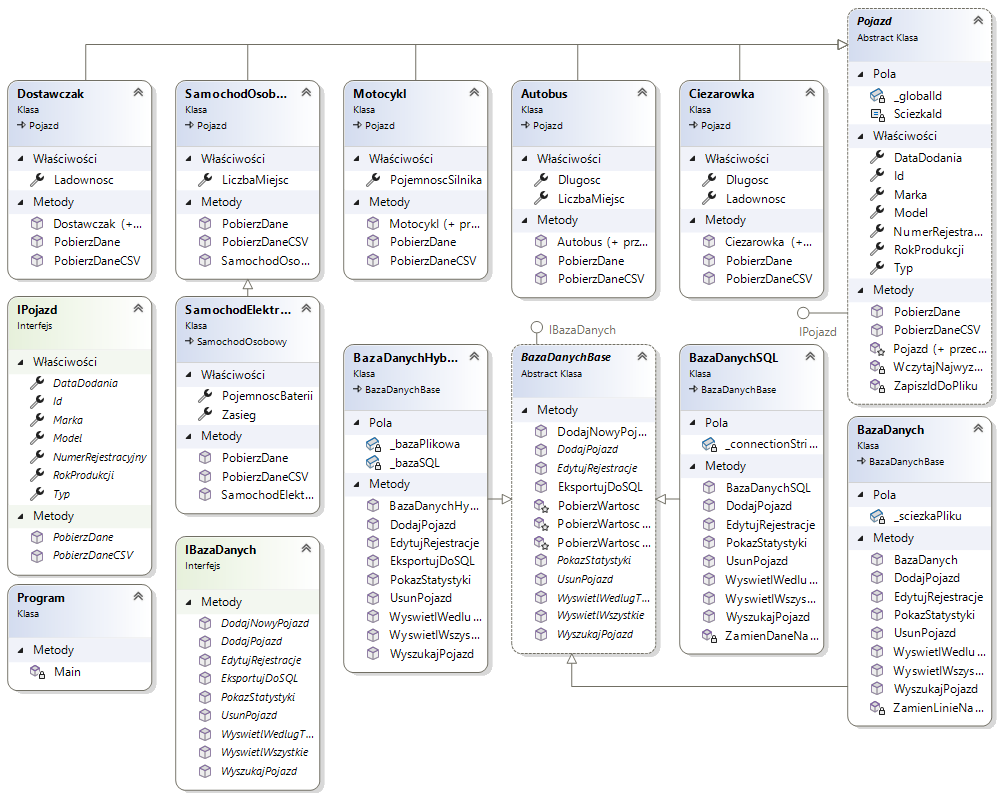
\includegraphics[width=1\textwidth]{Diagram klas.png}
    \caption{Diagram klas}
    \label{fig:moj_obrazek}
\end{figure}
\section{Opis najważniejszych metod}
\begin{itemize}
    \item DodajPojazd(IPojazd pojazd) – dodaje pojazd do bazy danych.
    \item UsunPojazd(string rejestracja) – usuwa pojazd na podstawie numeru rejestracyjnego.
    \item EdytujRejestracje(string staraRejestracja, string nowaRejestracja) – zmienia numer rejestracyjny pojazdu.
    \item WyszukajPojazd(string rejestracja) – wyszukuje pojazd po numerze rejestracyjnym.
    \item WyswietlWszystkie() – zwraca listę wszystkich pojazdów.
    \item WyswietlWedlugTypu(string typ) – zwraca listę pojazdów danego typu.
    \item PokazStatystyki() – generuje statystyki na podstawie danych.
    \item EksportujDoSQL(IBazaDanych sqlBaza) – eksportuje dane z plików TXT do bazy SQL.
\end{itemize}
\newpage
% ********** Rozdział 4 **********
\chapter{Harmonogram realizacji projektu}
Realizacja projektu "Zarządzanie pojazdami" została zaplanowana i przeprowadzona zgodnie z harmonogram realizacji projektu oparrtym na diagram Gantta. Przedstawia on poszczególne etapy projektu rozłożone w czasie.


\begin{figure}[h] 
    \centering
    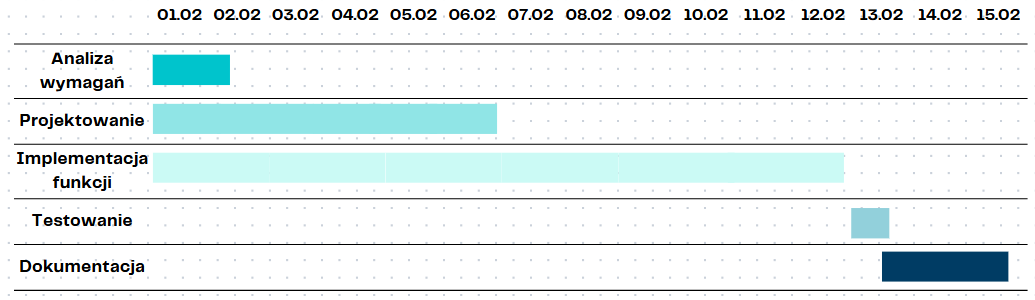
\includegraphics[width=1\textwidth]{Daigram gaunt.png}
    \caption{Diagram Gauntta}
    \label{fig:moj_obrazek}
\end{figure}
Etapy realizacji projektu na podstawie diagramu Gantta:
\begin{itemize}
    \item Analiza wymagań – określenie funkcjonalności i wymagań projektu.
    \item Projektowanie systemu – zaprojektowanie struktury klas, interfejsów i diagramu klas.
    \item Implementacja systemu – implementacja klas, interfejsów i testowanie funkcjonalności.
    \item Testowanie systemu – sprawdzenie poprawności działania systemu i naprawa błędów.
    \item Dokumentacja projektu – przygotowanie dokumentacji technicznej i użytkownika.
\end{itemize}
\section*{Repozytoriun i system kontroli wersji}
Projekt został zrealizowany z wykorzystaniem systemu kontroli wersji Git oraz platformy GitHub. Repozytorium projektu znajduje się pod adresem: \url{https://github.com/w69760/Labolatoria}
% ********** Koniec rozdziału **********
\newpage
% ********** Rozdział 4 **********
\chapter{Prezentacja warstwy użytkowej projektu}

\section{Opis warstwy użytkowej}
Warstwa użytkowa w omawianej aplikacji została zaimplementowana 
w postaci konsolowego programu (\texttt{Program.cs}). Użytkownik wchodzi w interakcję 
z systemem poprzez menu wyświetlane w konsoli, w którym dostępne są następujące opcje:
\begin{figure}[H] 
    \centering
    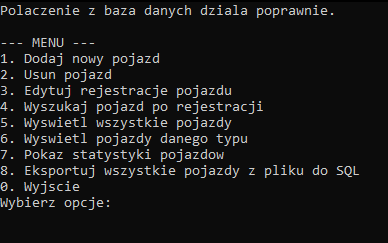
\includegraphics[width=1\textwidth]{ManuGlowne.png}
    \caption{Menu główne aplikacji}
    \label{fig:moj_obrazek}
\end{figure}
\begin{itemize}
    \item \textbf{Dodawanie nowego pojazdu} -- użytkownik wprowadza dane pojazdu (marka, model, rok itp.), 
    a program wywołuje odpowiednie metody warstwy dostępowej do bazy (np. \texttt{DodajNowyPojazd}).
    \begin{figure}[H] 
        \centering
        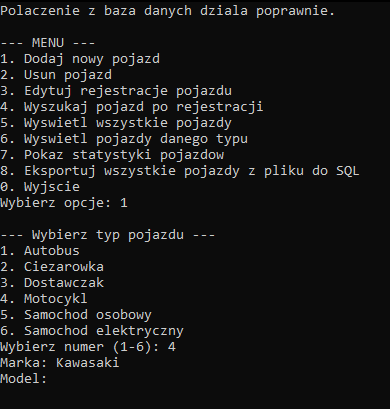
\includegraphics[width=1\textwidth]{Dodawanie.png}
        \caption{Dodawanie pojazdu}
        \label{fig:moj_obrazek}
    \end{figure}
    \item \textbf{Usuwanie pojazdu} -- użytkownik podaje numer rejestracyjny, a aplikacja usuwa pojazd 
    z bazy plikowej i bazy SQL.
    \begin{figure}[H] 
        \centering
        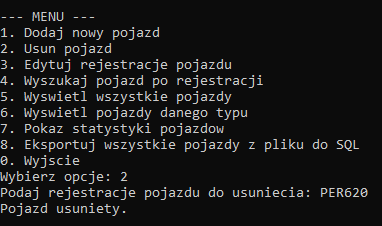
\includegraphics[width=1\textwidth]{Usuwanie.png}
        \caption{Usuwanie pojazdu}
        \label{fig:moj_obrazek}
    \end{figure}
    \item \textbf{Edycja rejestracji} -- umożliwia zmianę numeru rejestracyjnego istniejącego pojazdu.
    \begin{figure}[H] 
        \centering
        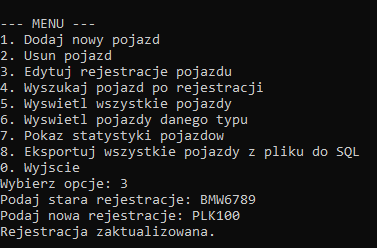
\includegraphics[width=1\textwidth]{Rejestracja.png}
        \caption{Edycja rejestracji}
        \label{fig:moj_obrazek}
    \end{figure}
    \item \textbf{Wyszukiwanie pojazdu} -- na podstawie rejestracji program wyświetla informacje 
    o odnalezionym pojeździe (lub komunikat o braku pojazdu).
    \begin{figure}[H] 
        \centering
        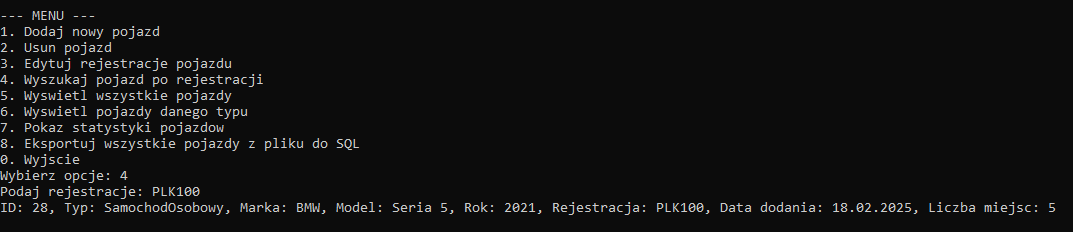
\includegraphics[width=1\textwidth]{WyszukiwanieRejestracja.png}
        \caption{Wyszukiwanie pojazdu po numerze rejestracyjnym}
        \label{fig:moj_obrazek}
    \end{figure}
    \item \textbf{Wyświetlanie pojazdów} -- aplikacja pobiera listę wszystkich pojazdów z warstwy dostępowej 
    i prezentuje je w konsoli.
    \begin{figure}[H] 
        \centering
        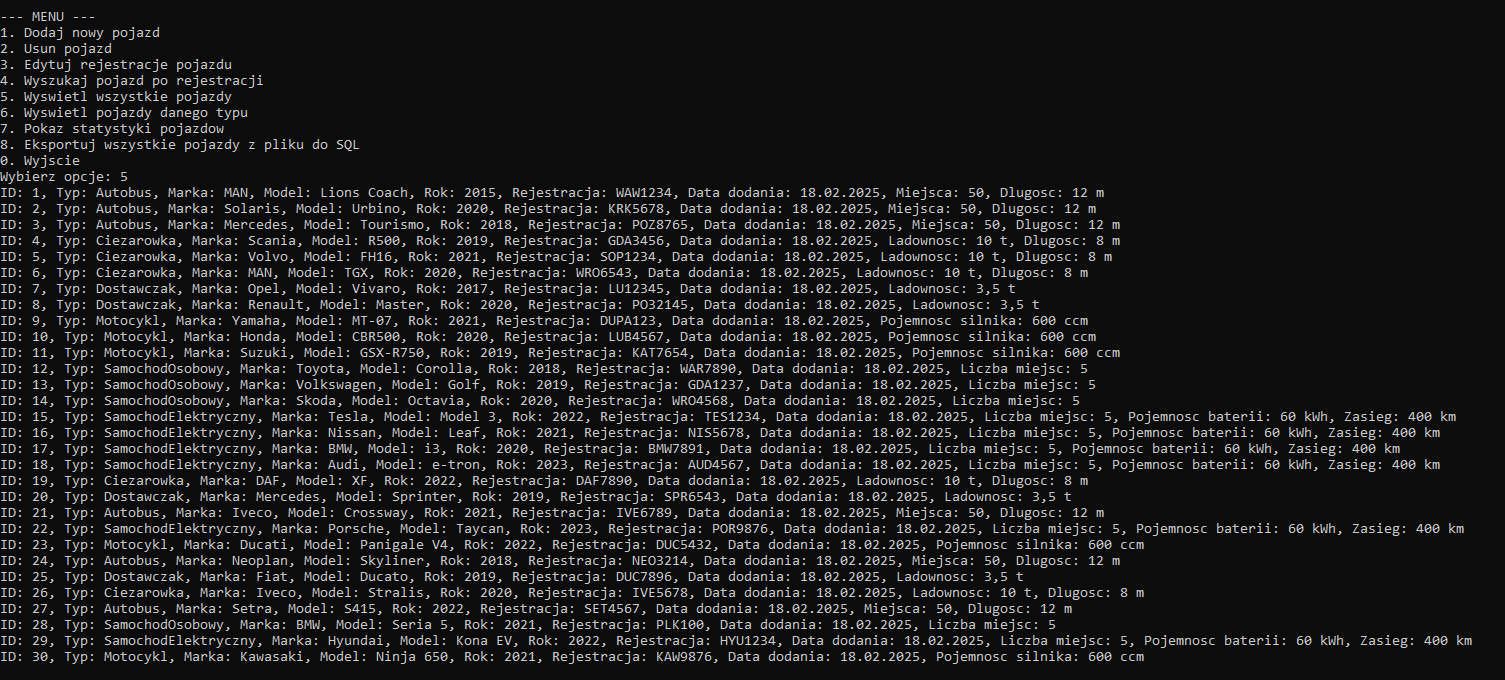
\includegraphics[width=1\textwidth]{Wyswietlanie wszyskiego.png}
        \caption{Wyświetlanie wszystkich pojazdów}
        \label{fig:moj_obrazek}
    \end{figure}
    \item \textbf{Wyświetlanie pojazdów danego typu} -- użytkownik wybiera typ (np. \textit{Autobus}, 
    \textit{Ciezarowka}, \textit{Motocykl}), a program wyświetla pasujące rekordy.
    \begin{figure}[H] 
        \centering
        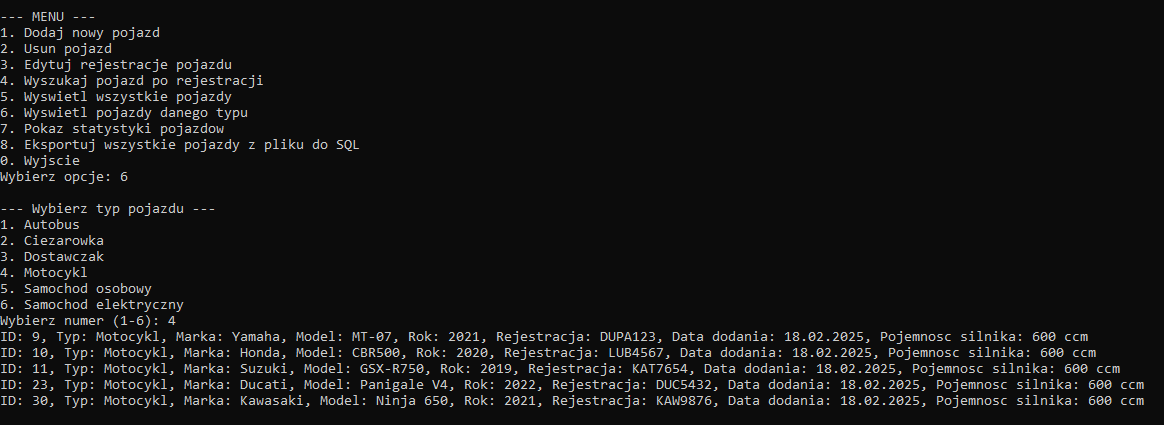
\includegraphics[width=1\textwidth]{DanyTyp.png}
        \caption{Wyswietlanie danego typu pojazdow}
        \label{fig:moj_obrazek}
    \end{figure}
    \item \textbf{Statystyki} -- pozwala na wyświetlenie informacji statystycznych (np. liczba pojazdów 
    w każdej kategorii).
    \begin{figure}[H] 
        \centering
        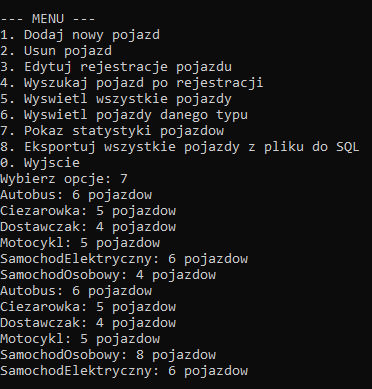
\includegraphics[width=1\textwidth]{Statystyki.png}
        \caption{Statystyki pojazdów}
        \label{fig:moj_obrazek}
    \end{figure}
    \item \textbf{Eksport do SQL} -- umożliwia przeniesienie danych z bazy plikowej do bazy SQL 
    (z zachowaniem walidacji).
    \begin{figure}[H] 
        \centering
        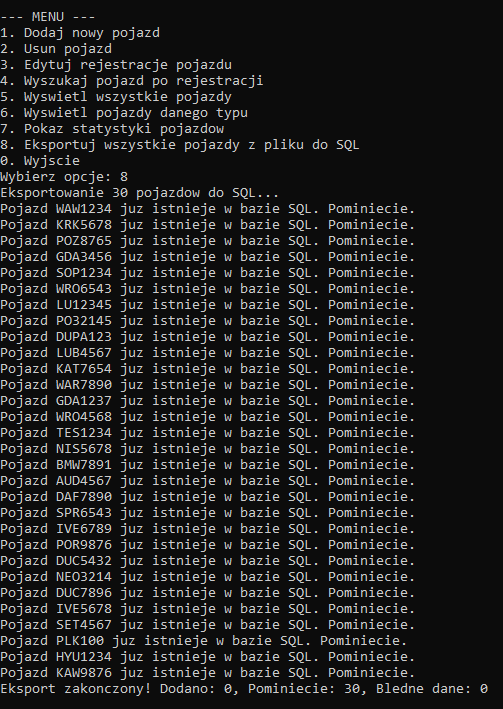
\includegraphics[width=1\textwidth]{Eksport.png}
        \caption{Eksport danych do SQL}
        \label{fig:moj_obrazek}
    \end{figure}
\end{itemize}

\subsection{Sposób działania}
Cała komunikacja z użytkownikiem odbywa się w pętli \texttt{while}, która wyświetla menu 
i w zależności od wybranej opcji wywołuje konkretne metody warstwy dostępowej. 
Dzięki temu warstwa użytkowa jest odpowiedzialna wyłącznie za:
\begin{enumerate}
    \item Pobieranie danych wejściowych od użytkownika,
    \item Wywoływanie metod z warstwy logiki/baz danych (np. \texttt{DodajPojazd}, \texttt{UsunPojazd}),
    \item Prezentację wyników w konsoli (np. listy pojazdów, komunikaty o błędach).
\end{enumerate}

\subsection{Zalety podejścia}
\begin{itemize}
    \item \textbf{Oddzielenie logiki biznesowej od interfejsu} -- kod obsługujący dane i bazę jest w odrębnych klasach, 
    co ułatwia modyfikacje i testy.
    \item \textbf{Łatwa rozbudowa} -- w przyszłości można zastąpić interfejs konsolowy np. interfejsem graficznym, 
    bez konieczności modyfikowania metod logiki lub bazy danych.
    \item \textbf{Przejrzystość} -- menu konsolowe jest intuicyjne w obsłudze, a kolejne opcje (dodawanie, usuwanie, 
    wyszukiwanie) są jasno wyodrębnione.
\end{itemize}

\section{Podsumowanie}
Warstwa użytkowa w postaci aplikacji konsolowej stanowi prosty, ale skuteczny sposób 
na interakcję z systemem \textbf{ZarządzaniePojazdami}. Dzięki czytelnej strukturze menu 
oraz wywoływaniu metod z warstwy logiki i dostępu do danych, użytkownik może w łatwy sposób 
dodawać, usuwać, modyfikować i przeglądać pojazdy w bazie.




\newpage
% ********** Rozdział 4 **********
\chapter{Podsumowanie}

W niniejszym rozdziale przedstawiono zrealizowane prace związane z projektem oraz kierunki dalszego rozwoju systemu.

\section{Zrealizowane prace}
W ramach projektu udało się zrealizować następujące elementy:
\begin{itemize}
    \item Stworzenie wielowarstwowej architektury aplikacji, obejmującej warstwę dostępu do danych oraz interfejs użytkownika.
    \item Implementacja systemu zarządzania pojazdami, w tym obsługa dodawania, usuwania, edycji rejestracji, wyszukiwania oraz wyświetlania pojazdów.
    \item Integracja danych z dwóch źródeł – bazy plikowej i bazy SQL – umożliwiająca eksport danych oraz synchronizację między nimi.
    \item Opracowanie konsolowego interfejsu użytkownika, który zapewnia intuicyjną obsługę systemu poprzez menu oraz wizualizację operacji (poprzez dołączone zrzuty ekranu).
    \item Zabezpieczenie operacji na danych poprzez implementację odpowiednich walidacji oraz obsługi wyjątków.
\end{itemize}

\section{Planowane dalsze prace rozwojowe}
W kolejnych etapach rozwoju projektu planowane są następujące działania:
\begin{itemize}
    \item Rozszerzenie funkcjonalności interfejsu użytkownika poprzez wdrożenie graficznego interfejsu (GUI), co umożliwi bardziej przyjazną interakcję z systemem.
    \item Ulepszenie mechanizmu walidacji danych i obsługi błędów, aby zwiększyć niezawodność aplikacji w środowisku produkcyjnym.
    \item Integracja systemu z nowoczesnymi rozwiązaniami bazodanowymi oraz API, co pozwoli na lepszą skalowalność i integrację z innymi systemami.
    \item Przeprowadzenie testów wydajnościowych oraz optymalizacja operacji na dużych zbiorach danych, aby zapewnić szybki dostęp do informacji.
    \item Rozwój modułu raportowania i analizy statystyk, co umożliwi generowanie szczegółowych raportów oraz lepsze podejmowanie decyzji na podstawie zgromadzonych danych.
\end{itemize}


% ********** Koniec rozdziału **********


\newpage
\input{R6.tex}
\newpage



% *************** Zakończenie ***************
% *************** Zakończenie ***************

%***************************************************************************************
% W tym miejscu znajdują się polecenia odpowiedzialne za tworzenie
% spisu ilustracji, spisu treści oraz streszczenia pracy
%***************************************************************************************

%spis rysunków
\addcontentsline{toc}{chapter}{Spis rysunków}
\listoffigures
\newpage



% %streszczenie
% \addcontentsline{toc}{chapter}{Streszczenie}
% \noindent
% {\footnotesize{}\textbf{Wyższa Szkoła Informatyki i Zarządzania z siedzibą w Rzeszowie\\
% Kolegium Informatyki Stosowanej}
% \vspace{30pt}

% \begin{center}
% \textbf{Streszczenie pracy dyplomowej inżynierskiej}\\
% \temat
% \end{center}

% \vspace{30pt}
% \noindent
% \textbf{Autor: \autor
% \\Promotor: \promotor
% \\Słowa kluczowe: tutaj umieść słowa kluczowe}
% \vspace{40pt}
% \\Treść streszczenia, czyli kilka zdań dotyczących treści pracy dyplomowej w języku polskim.
% \vspace{80pt}

% \noindent
% \textbf{The University of Information Technology and Management in Rzeszow\\
% Faculty of Applied Information Technology}
% \vspace{30pt}

% \begin{center}
% \textbf{Thesis Summary\\}
% Tytuł pracy w języku angielskim
% \end{center}

% \vspace{30pt}
% \noindent
% \textbf{Author: \autor
% \\Supervisor: \promotor
% \\Key words: tutaj umieść słowa kluczowe}
% \vspace{40pt}
% \\Treść streszczenia, czyli kilka zdań dotyczących treści pracy dyplomowej w języku angielskim - tłumaczenie tekstu z języka polskiego.
% }

% *************** Koniec pliku back.tex ***************


\end{document}
% *************** Koniec pliku szablon.tex ***************
